\section{Лекция 4. Критерий единственности решения задачи Коши для автономного дифференциального уравнения}
\noeqref{eq:l4_aut_ode, eq:l4_criterion, eq:l4_ex1_ode, eq:l4_ex2_ode}
\noeqref{eq:l4_ex3_ode}

\begin{flushright}
    28.09.26
\end{flushright}

\subsection{Критерий единственности для автономного уравнения 1-го порядка}

Рассмотрим частный класс уравнений с разделяющимися переменными, правая часть
которых явно не зависит от независимой переменной $x$.

\begin{definition}
    \textdef{Автономным} называется дифференциальное уравнение вида:
    \begin{equation} \label{eq:l4_aut_ode}
        y' = f(y), \tag{1}
    \end{equation}
    где $f \in C(I)$ — непрерывная на интервале $I \subset \R$ функция.
\end{definition}

Если в некоторой точке $y = C \in I$ правая часть обращается в нуль
($f(C) = 0$), то постоянная функция $y(x) \equiv C$ является решением уравнения
\eqref{eq:l4_aut_ode}, которое называется \textdef{стационарным решением} (или
\textdef{положением равновесия}).

Если в точке $y = C$ функция $f(y)$ удовлетворяет условию Липшица (например,
имеет конечную производную $f'(C)$), то по теореме Пикара из Лекции 3 через
любую точку прямой $y = C$ проходит единственное решение, и $y \equiv C$
особым решением быть не может. Однако если условие Липшица в точке $y = C$
нарушается, возникает фундаментальный вопрос: \textbf{является ли стационарное
решение $y \equiv C$ особым} (в смысле определения 2.2 из Лекции 2)? Ответ даёт
следующий точный критерий.

\begin{theorem}[\textbf{Критерий единственности (Осгуда) для автономного ОДУ}]
    Пусть $y \equiv C$ — изолированное стационарное решение автономного
    уравнения \eqref{eq:l4_aut_ode}, то есть $f(C) = 0$ и $f(y) \neq 0$ в
    проколотой окрестности точки $C$. Решение $y \equiv C$ является
    \textdef{особым} тогда и только тогда, когда хотя бы с одной стороны от
    точки $C$ сходится несобственный интеграл:
    \begin{equation} \label{eq:l4_criterion}
        \int_{y_0}^{C} \frac{dy}{f(y)}. \tag{2}
    \end{equation}
    Если же интеграл \eqref{eq:l4_criterion} расходится, то $y \equiv C$
    особым решением не является, и единственность решения задачи Коши на прямой
    $y = C$ сохраняется.
\end{theorem}

\begin{proof}[Обоснование критерия]~\\
    \begin{quote}
        Выберем начальную точку $(x_0, y_0)$ так, чтобы на полуинтервале
        $[y_0, C)$ функция $f(y)$ не имела нулей: $f(y) \neq 0$. Разделим
        переменные в уравнении \eqref{eq:l4_aut_ode} и проинтегрируем от
        $(x_0, y_0)$ до текущей точки $(x, y)$:
        \[
            \frac{dy}{f(y)} = dx \implies
            \int_{y_0}^{y} \frac{d\xi}{f(\xi)} = \int_{x_0}^{x} d\tau \implies
            x(y) = x_0 + \int_{y_0}^{y} \frac{d\xi}{f(\xi)}.
        \]
        Выясним, может ли эта интегральная кривая достигнуть горизонтальной
        прямой $y = C$ при конечном значении абсциссы $x = x^*$. Перейдём к
        пределу при $y \to C$:
        \[
            x^* = \lim_{y \to C} x(y) = x_0 + \int_{y_0}^{C} \frac{d\xi}{f(\xi)}.
        \]
        Возможны два случая:
        \begin{itemize}
            \item \textbf{Интеграл \eqref{eq:l4_criterion} сходится.} Тогда
            предельное значение $x^* \in \R$ конечно, и интегральная кривая
            примыкает к прямой $y = C$ в точке $(x^*, C)$. Поскольку уравнение
            \eqref{eq:l4_aut_ode} автономно, оно инвариантно относительно
            сдвигов вдоль оси $Ox$ ($x \mapsto x + \text{const}$). Сдвигая
            найденную кривую вдоль оси абсцисс, мы получим семейство решений,
            примыкающих к прямой $y = C$ в каждой её точке. Следовательно,
            единственность всюду на $y = C$ нарушается, и $y \equiv C$ —
            \textdef{особое решение}.
            \item \textbf{Интеграл \eqref{eq:l4_criterion} расходится.} Тогда
            $\abs{x^*} = \infty$, то есть интегральная кривая приближается к
            прямой $y = C$ лишь асимптотически при $x \to \pm\infty$, не
            пересекая её ни в одной конечной точке. Единственность не
            нарушается, и $y \equiv C$ \textdef{не является особым решением}.
        \end{itemize}
    \end{quote}
\end{proof}

\subsection{Разбор характерных примеров}

\begin{example}
    Исследовать на наличие особых решений уравнение:
    \begin{equation} \label{eq:l4_ex1_ode}
        y' = y^{1/3}. \tag{3}
    \end{equation}

    \begin{proof}[Решение]~\\
        \begin{quote}
            Правая часть $f(y) = y^{1/3} \in C(\R)$ обращается в нуль при
            $y = 0$, причём $f'(y) = \frac{1}{3} y^{-2/3} \to \infty$ при
            $y \to 0$ (условие Липшица в нуле нарушено).

            Проверим стационарное решение $y \equiv 0$ по критерию
            \eqref{eq:l4_criterion}:
            \[
                \int_{y_0}^{0} \frac{dy}{y^{1/3}} =
                \int_{y_0}^{0} y^{-1/3} \, dy =
                \left. \frac{3}{2} y^{2/3} \right|_{y_0}^{0} =
                -\frac{3}{2} y_0^{2/3} \in \R.
            \]
            Поскольку показатель степени $1/3 < 1$, несобственный интеграл
            \textbf{сходится}. Следовательно, $y \equiv 0$ — \textdef{особое
            решение}.

            Найдём остальные интегральные кривые при $y \neq 0$:
            \[
                y^{-1/3} \, dy = dx \implies \frac{3}{2} y^{2/3} = x + C
                \implies y(x) = \pm \left(\frac{2}{3}(x + C)\right)^{3/2},
                \quad x \ge -C.
            \]
            Каждая полукубическая парабола этого семейства касается прямой
            $y = 0$ в точке $x = -C$.
        \end{quote}
    \end{proof}
\end{example}

\begin{figure}[H]
    \centering
    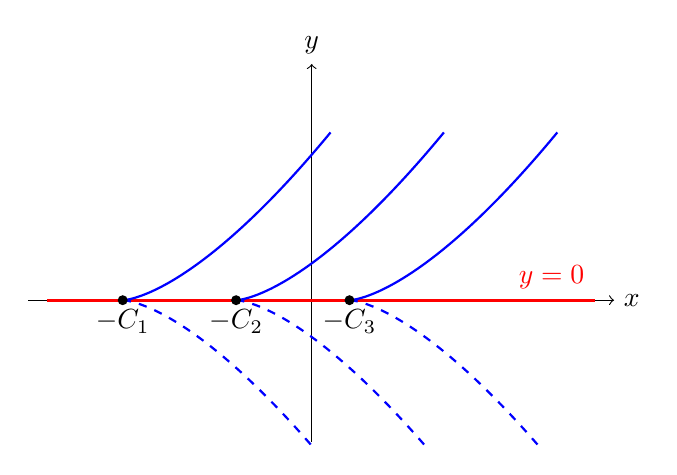
\begin{tikzpicture}[scale=1.2]
        % Оси координат
        \draw[->] (-3.0, 0) -- (3.2, 0) node[right] {$x$};
        \draw[->] (0, -1.5) -- (0, 2.5) node[above] {$y$};

        % Особое решение y = 0
        \draw[red, very thick] (-2.8, 0) -- (3.0, 0)
            node[above left, red] {$y = 0$};

        % Ветви полукубических парабол
        \foreach \c/\lbl in {-2/C_1, -0.8/C_2, 0.4/C_3} {
            \draw[blue, thick, domain=\c:\c+2.2, samples=60]
                plot (\x, {(2/3*(\x - \c))*sqrt(2/3*(\x - \c))});
            \draw[blue, thick, dashed, domain=\c:\c+2.0, samples=60]
                plot (\x, {-(2/3*(\x - \c))*sqrt(2/3*(\x - \c))});
            \fill[black] (\c, 0) circle (1.5pt) node[below] {$-\lbl$};
        }
    \end{tikzpicture}
    \caption{Семейство интегральных кривых уравнения $y' = y^{1/3}$,
    примыкающих к особому решению $y = 0$ в точках $x = -C_i$.}
\end{figure}

\begin{example}
    Исследовать на наличие особых решений уравнение:
    \begin{equation} \label{eq:l4_ex2_ode}
        y' =
        \begin{cases}
            y \ln y, & y > 0, \\
            0, & y = 0.
        \end{cases} \tag{4}
    \end{equation}

    \begin{proof}[Решение]~\\
        \begin{quote}
            Как было доказано в контрпримере из Лекции 2 (раздел 2.3), правая
            часть $f(y)$ непрерывна на $[0, +\infty)$, но \textbf{не
            удовлетворяет условию Липшица} в окрестности точки $y = 0$.
            Уравнение $f(y) = 0$ даёт два стационарных решения: $y \equiv 0$ и
            $y \equiv 1$. Исследуем оба положения равновесия по критерию
            \eqref{eq:l4_criterion} (при $y_0 \in (0, 1)$):

            \textbf{1. Проверка решения $y \equiv 0$:}
            \[
                \int_{y_0}^{0} \frac{dy}{y \ln y} =
                \lim_{\eps \to +0} \int_{y_0}^{\eps} \frac{d(\ln y)}{\ln y} =
                \lim_{\eps \to +0} \left. \ln \abs{\ln y} \right|_{y_0}^{\eps}
                = +\infty.
            \]
            Интеграл \textbf{расходится}. Следовательно, несмотря на нарушение
            условия Липшица в нуле, прямая $y \equiv 0$ \textdef{не является
            особым решением}!

            \textbf{2. Проверка решения $y \equiv 1$:}
            \[
                \int_{y_0}^{1} \frac{dy}{y \ln y} =
                \lim_{\eps \to 1-0} \left. \ln \abs{\ln y} \right|_{y_0}^{\eps}
                = -\infty.
            \]
            Интеграл также \textbf{расходится}, поэтому $y \equiv 1$
            \textdef{не является особым решением} (что согласуется и с
            теоремой Пикара, так как $f'(1) = 1 < \infty$).
        \end{quote}
    \end{proof}
\end{example}

\begin{figure}[H]
    \centering
    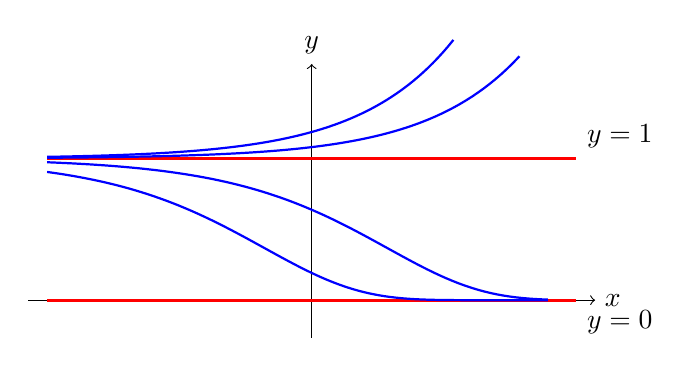
\begin{tikzpicture}[scale=1.2]
        % Оси координат
        \draw[->] (-3.0, 0) -- (3.0, 0) node[right] {$x$};
        \draw[->] (0, -0.4) -- (0, 2.5) node[above] {$y$};

        % Стационарные решения y = 0 и y = 1
        \draw[red, very thick] (-2.8, 0) -- (2.8, 0)
            node[below right, black] {$y = 0$};
        \draw[red, very thick] (-2.8, 1.5) -- (2.8, 1.5)
            node[above right, black] {$y = 1$};

        % Интегральные кривые выше y = 1
        \draw[blue, thick, domain=-2.8:2.2, samples=80]
            plot (\x, {1.5 + 0.12*exp(\x)});
        \draw[blue, thick, domain=-2.8:1.5, samples=80]
            plot (\x, {1.5 + 0.28*exp(\x)});

        % Интегральные кривые в полосе 0 < y < 1: y = exp(-exp(x + C))
        \draw[blue, thick, domain=-2.8:2.5, samples=80]
            plot (\x, {1.5 * exp(-exp(\x - 0.8))});
        \draw[blue, thick, domain=-2.8:2.5, samples=80]
            plot (\x, {1.5 * exp(-exp(\x + 0.5))});
    \end{tikzpicture}
    \caption{Интегральные кривые уравнения $y' = y \ln y$: все нестационарные
    решения приближаются к прямым $y = 0$ и $y = 1$ лишь асимптотически при
    $x \to \pm\infty$.}
\end{figure}

\begin{example}
    Исследовать на наличие особых решений уравнение:
    \begin{equation} \label{eq:l4_ex3_ode}
        y' =
        \begin{cases}
            y \ln^2 y, & y > 0, \\
            0, & y = 0.
        \end{cases} \tag{5}
    \end{equation}

    \begin{proof}[Решение]~\\
        \begin{quote}
            Стационарные решения те же: $y \equiv 0$ и $y \equiv 1$. Вычислим
            несобственные интегралы \eqref{eq:l4_criterion} при
            $y_0 \in (0, 1)$:

            \textbf{1. Проверка решения $y \equiv 0$:}
            \[
                \int_{y_0}^{0} \frac{dy}{y \ln^2 y} =
                \lim_{\eps \to +0} \int_{y_0}^{\eps} \frac{d(\ln y)}{\ln^2 y} =
                \lim_{\eps \to +0} \left. \left(-\frac{1}{\ln y}\right)
                \right|_{y_0}^{\eps} = 0 + \frac{1}{\ln y_0} =
                \frac{1}{\ln y_0} \in \R.
            \]
            Интеграл \textbf{сходится}! Следовательно, $y \equiv 0$
            \textdef{является особым решением}: интегральные кривые вида
            $y(x) = \exp\left(-\frac{1}{x + C}\right)$ в полосе $0 < y < 1$
            примыкают к прямой $y = 0$ слева при конечных значениях $x = -C$.

            \textbf{2. Проверка решения $y \equiv 1$:}
            \[
                \int_{y_0}^{1} \frac{dy}{y \ln^2 y} =
                \lim_{\eps \to 1-0} \left. \left(-\frac{1}{\ln y}\right)
                \right|_{y_0}^{\eps} = +\infty.
            \]
            Интеграл \textbf{расходится}, поэтому $y \equiv 1$ \textdef{не
            является особым решением}.
        \end{quote}
    \end{proof}
\end{example}

\begin{figure}[H]
    \centering
    \begin{tikzpicture}[scale=1.2]
        % Оси координат
        \draw[->] (-3.0, 0) -- (3.2, 0) node[right] {$x$};
        \draw[->] (0, -0.4) -- (0, 2.2) node[above] {$y$};

        % Стационарные решения
        \draw[red, very thick] (-2.8, 0) -- (3.0, 0)
            node[below right, red] {$y = 0$ (особое)};
        \draw[teal, very thick] (-2.8, 1.6) -- (3.0, 1.6)
            node[above right, teal] {$y = 1$ (не особое)};

        % Кривые в полосе 0 < y < 1, касающиеся y = 0 в точках x = -C_i
        \foreach \c/\lbl in {-0.8/C_1, 0.6/C_2, 2.0/C_3} {
            \draw[blue, thick, domain=-2.8:\c-0.08, samples=80]
                plot (\x, {1.6 * exp(1/(\x - \c))});
            \fill[black] (\c, 0) circle (1.5pt) node[below] {$-\lbl$};
        }
    \end{tikzpicture}
    \caption{Интегральные кривые уравнения $y' = y \ln^2 y$ в полосе
    $0 < y < 1$: слева ($x \to -\infty$) они асимптотически стремятся к
    $y = 1$, а справа достигают особого решения $y = 0$ в конечных точках
    $x = -C_i$.}
\end{figure}

\begin{remark}
    Для самостоятельной отработки критерия единственности рекомендуется
    решить задачи № 51, 52, 53, 55 и 56 из задачника А. Ф. Филиппова.
\end{remark}